% ==========================================================================
% INFO 4617 Web Data Science -- Week 5: Web Architecture & Protocols (Chapter 5)
% Build:  latexmk -pdf week-05.tex   (from this folder; no env vars needed)
% (or run `make` from the slides/ directory to build every deck)
% ==========================================================================
\documentclass[9pt,aspectratio=169]{beamer}
% Resolve the shared theme/preamble in ../common/ when compiling this
% file directly from its own folder (no TEXINPUTS needed).
\makeatletter\def\input@path{{../common/}}\makeatother
% ==========================================================================
% Shared preamble for INFO 4617 Web Data Science weekly lecture decks
% Based on the Gotham beamer theme (vendored in this directory).
% Each week's slides.tex does:  % ==========================================================================
% Shared preamble for INFO 4617 Web Data Science weekly lecture decks
% Based on the Gotham beamer theme (vendored in this directory).
% Each week's slides.tex does:  % ==========================================================================
% Shared preamble for INFO 4617 Web Data Science weekly lecture decks
% Based on the Gotham beamer theme (vendored in this directory).
% Each week's slides.tex does:  \input{preamble}  (with common/ on TEXINPUTS)
% then sets \title/\subtitle/\author/\date and \begin{document}.
% ==========================================================================

\usetheme{gotham}

\usepackage{fbb}
\usepackage{booktabs}
\usepackage{graphicx}
\usepackage{tikz}
\usepackage{xcolor}
\usepackage{multirow}
\usepackage{listings}
\usetikzlibrary{positioning, arrows.meta, shapes}

% Bibliography
\usepackage[style=authoryear,
            backend=biber,
            maxcitenames=1,
            uniquename=false,
            uniquelist=false]{biblatex}
\addbibresource{bibliography.bib}

\gothamset{sectiontocframe default=off}

% ------------------------------------------------------------------ colors
\definecolor{cugold}{HTML}{CFB87C}
\definecolor{tab-red}{HTML}{E15759}
\definecolor{tab-orange}{HTML}{F28E2B}
\definecolor{tab-blue}{HTML}{4E79A7}
\definecolor{tab-cyan}{HTML}{76B7B2}
\definecolor{tab-green}{HTML}{59A14F}
\definecolor{tab-yellow}{HTML}{EDC948}
\definecolor{tab-purple}{HTML}{B07AA1}
\definecolor{tab-pink}{HTML}{FF9DA7}
\definecolor{tab-brown}{HTML}{9C755F}
\definecolor{tab-gray}{HTML}{BAB0AC}

\setbeamercolor{frametitle}{fg=black, bg=cugold}
\setbeamercolor{progress bar}{fg=cugold, bg=cugold!20}

\setbeamercolor{block title alerted}{fg=black, bg=cugold}
\setbeamercolor{block body alerted}{fg=black, bg=cugold!10}

% ------------------------------------------------------------------ footline
\setbeamertemplate{footline}{
  \begin{beamercolorbox}[wd=\paperwidth,ht=2.5ex,dp=1ex,right]{footline}
    {\footnotesize \insertframenumber{} of \inserttotalframenumber}
    \hspace*{2ex}
  \end{beamercolorbox}
}

% ------------------------------------------------------------------ helpers
\newcommand{\bottomcite}[1]{
    \vspace*{\fill}
    \vspace{-\baselineskip}
    {\tiny
    \rule{\textwidth}{0.3pt}\\
    #1
    }
    \vspace{0.5ex}
}

% Consistent code styling for the Wednesday "applied notebook" frames.
\lstdefinestyle{wds}{
    basicstyle=\ttfamily\scriptsize,
    keywordstyle=\color{tab-blue}\bfseries,
    commentstyle=\color{tab-green},
    stringstyle=\color{tab-orange},
    showstringspaces=false,
    breaklines=true,
    columns=fullflexible,
    language=Python,
    aboveskip=0.4em,
    belowskip=0.4em,
}
\lstset{style=wds}

% \dayband{Day}{Topic} -- a lightweight section divider label used to mark
% Monday / Wednesday / Friday within a week's deck.
\newcommand{\dayband}[2]{{\large\textbf{#1}}\;\textcolor{tab-gray}{\textbar}\;#2}
  (with common/ on TEXINPUTS)
% then sets \title/\subtitle/\author/\date and \begin{document}.
% ==========================================================================

\usetheme{gotham}

\usepackage{fbb}
\usepackage{booktabs}
\usepackage{graphicx}
\usepackage{tikz}
\usepackage{xcolor}
\usepackage{multirow}
\usepackage{listings}
\usetikzlibrary{positioning, arrows.meta, shapes}

% Bibliography
\usepackage[style=authoryear,
            backend=biber,
            maxcitenames=1,
            uniquename=false,
            uniquelist=false]{biblatex}
\addbibresource{bibliography.bib}

\gothamset{sectiontocframe default=off}

% ------------------------------------------------------------------ colors
\definecolor{cugold}{HTML}{CFB87C}
\definecolor{tab-red}{HTML}{E15759}
\definecolor{tab-orange}{HTML}{F28E2B}
\definecolor{tab-blue}{HTML}{4E79A7}
\definecolor{tab-cyan}{HTML}{76B7B2}
\definecolor{tab-green}{HTML}{59A14F}
\definecolor{tab-yellow}{HTML}{EDC948}
\definecolor{tab-purple}{HTML}{B07AA1}
\definecolor{tab-pink}{HTML}{FF9DA7}
\definecolor{tab-brown}{HTML}{9C755F}
\definecolor{tab-gray}{HTML}{BAB0AC}

\setbeamercolor{frametitle}{fg=black, bg=cugold}
\setbeamercolor{progress bar}{fg=cugold, bg=cugold!20}

\setbeamercolor{block title alerted}{fg=black, bg=cugold}
\setbeamercolor{block body alerted}{fg=black, bg=cugold!10}

% ------------------------------------------------------------------ footline
\setbeamertemplate{footline}{
  \begin{beamercolorbox}[wd=\paperwidth,ht=2.5ex,dp=1ex,right]{footline}
    {\footnotesize \insertframenumber{} of \inserttotalframenumber}
    \hspace*{2ex}
  \end{beamercolorbox}
}

% ------------------------------------------------------------------ helpers
\newcommand{\bottomcite}[1]{
    \vspace*{\fill}
    \vspace{-\baselineskip}
    {\tiny
    \rule{\textwidth}{0.3pt}\\
    #1
    }
    \vspace{0.5ex}
}

% Consistent code styling for the Wednesday "applied notebook" frames.
\lstdefinestyle{wds}{
    basicstyle=\ttfamily\scriptsize,
    keywordstyle=\color{tab-blue}\bfseries,
    commentstyle=\color{tab-green},
    stringstyle=\color{tab-orange},
    showstringspaces=false,
    breaklines=true,
    columns=fullflexible,
    language=Python,
    aboveskip=0.4em,
    belowskip=0.4em,
}
\lstset{style=wds}

% \dayband{Day}{Topic} -- a lightweight section divider label used to mark
% Monday / Wednesday / Friday within a week's deck.
\newcommand{\dayband}[2]{{\large\textbf{#1}}\;\textcolor{tab-gray}{\textbar}\;#2}
  (with common/ on TEXINPUTS)
% then sets \title/\subtitle/\author/\date and \begin{document}.
% ==========================================================================

\usetheme{gotham}

\usepackage{fbb}
\usepackage{booktabs}
\usepackage{graphicx}
\usepackage{tikz}
\usepackage{xcolor}
\usepackage{multirow}
\usepackage{listings}
\usetikzlibrary{positioning, arrows.meta, shapes}

% Bibliography
\usepackage[style=authoryear,
            backend=biber,
            maxcitenames=1,
            uniquename=false,
            uniquelist=false]{biblatex}
\addbibresource{bibliography.bib}

\gothamset{sectiontocframe default=off}

% ------------------------------------------------------------------ colors
\definecolor{cugold}{HTML}{CFB87C}
\definecolor{tab-red}{HTML}{E15759}
\definecolor{tab-orange}{HTML}{F28E2B}
\definecolor{tab-blue}{HTML}{4E79A7}
\definecolor{tab-cyan}{HTML}{76B7B2}
\definecolor{tab-green}{HTML}{59A14F}
\definecolor{tab-yellow}{HTML}{EDC948}
\definecolor{tab-purple}{HTML}{B07AA1}
\definecolor{tab-pink}{HTML}{FF9DA7}
\definecolor{tab-brown}{HTML}{9C755F}
\definecolor{tab-gray}{HTML}{BAB0AC}

\setbeamercolor{frametitle}{fg=black, bg=cugold}
\setbeamercolor{progress bar}{fg=cugold, bg=cugold!20}

\setbeamercolor{block title alerted}{fg=black, bg=cugold}
\setbeamercolor{block body alerted}{fg=black, bg=cugold!10}

% ------------------------------------------------------------------ footline
\setbeamertemplate{footline}{
  \begin{beamercolorbox}[wd=\paperwidth,ht=2.5ex,dp=1ex,right]{footline}
    {\footnotesize \insertframenumber{} of \inserttotalframenumber}
    \hspace*{2ex}
  \end{beamercolorbox}
}

% ------------------------------------------------------------------ helpers
\newcommand{\bottomcite}[1]{
    \vspace*{\fill}
    \vspace{-\baselineskip}
    {\tiny
    \rule{\textwidth}{0.3pt}\\
    #1
    }
    \vspace{0.5ex}
}

% Consistent code styling for the Wednesday "applied notebook" frames.
\lstdefinestyle{wds}{
    basicstyle=\ttfamily\scriptsize,
    keywordstyle=\color{tab-blue}\bfseries,
    commentstyle=\color{tab-green},
    stringstyle=\color{tab-orange},
    showstringspaces=false,
    breaklines=true,
    columns=fullflexible,
    language=Python,
    aboveskip=0.4em,
    belowskip=0.4em,
}
\lstset{style=wds}

% \dayband{Day}{Topic} -- a lightweight section divider label used to mark
% Monday / Wednesday / Friday within a week's deck.
\newcommand{\dayband}[2]{{\large\textbf{#1}}\;\textcolor{tab-gray}{\textbar}\;#2}


\title[Week 5 · Protocols]{{\Huge Web Architecture \& Protocols}}
\subtitle{Week 5 · Foundations module · Textbook Chapter 5}
\author[Keegan]{\textbf{Brian C. Keegan, Ph.D.} \\ Associate Professor, Department of Information Science \\ University of Colorado Boulder}
\date{September 14, 16 \& 18, 2026}

\begin{document}

\maketitle

% -------------------------------------------------------------------------
\begin{frame}{This week at a glance}
    \begin{columns}[T]
        \begin{column}{0.6\textwidth}
            This week we examine the layers of protocols below the web. These layers turn a URL into a page on your screen. They also turn web data collection from \textit{magic} into \textit{engineering}.

            \bigskip

            \dayband{Monday}{Concepts \& notebook intro}
            \begin{itemize}\small
                \item Client--server, TCP/IP, DNS, and HTTP as one stack --- and how a server decides who, or what, is asking
                \item Close with a live pair activity: hunt for Inspector patterns across real sites
            \end{itemize}

            \medskip

            \dayband{Wednesday}{Notebook lab}
            \begin{itemize}\small
                \item Trace the stack in Python \emph{and} the terminal: a packet capture, a live API call, curl/wget
            \end{itemize}

            \medskip

            \dayband{Friday}{Textbook revisions}
            \begin{itemize}\small
                \item Propose \& peer-review pull requests improving Chapter 5
            \end{itemize}
        \end{column}
        \begin{column}{0.35\textwidth}
            \begin{block}{Companion notebook}
                \footnotesize \texttt{ch-05-protocols.ipynb}
            \end{block}
            \begin{alertblock}{Bring a laptop}
                \footnotesize Monday and Wednesday are both hands-on this week --- bring a laptop both days.
            \end{alertblock}
        \end{column}
    \end{columns}
\end{frame}

% =========================================================================
\section{Monday · Concepts}
% =========================================================================

\begin{frame}{ARPANET and the bomb}
    \begin{columns}[T]
        \begin{column}{0.55\textwidth}\small 
            Paul Baran (RAND, early 1960s) proposed \textbf{packet-switching} specifically so communications could survive a nuclear attack --- no single point of failure to knock out.

            \bigskip
            \textbf{ARPANET} (1969, DARPA) used packet-switching, but its real job was resource-sharing between expensive and inefficient research computers
            
            \bigskip
            \textbf{TCP/IP} (Cerf \& Kahn, 1970s) connected ARPANET to other, different networks, with robustness against unreliable or damaged links as a real design goal
            
            \bigskip
            The result is a decentralized network where packets route themselves around damage
        \end{column}
        \begin{column}{0.4\textwidth}
            \centering
            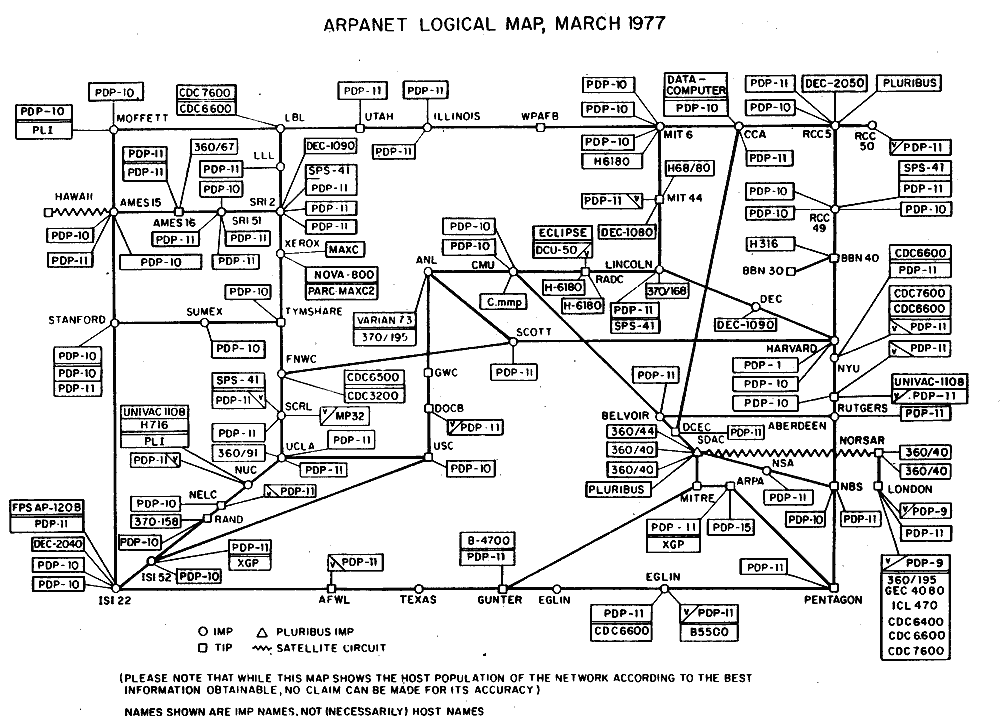
\includegraphics[width=\textwidth]{img/arpanet_map_1977.png}\\
            {\scriptsize ARPANET's actual topology, March 1977.}
        \end{column}
    \end{columns}
\end{frame}

\begin{frame}{Loading a web page, step by step}
    \begin{columns}[T]
        \begin{column}{0.6\textwidth}
            Type a URL, press Enter, and in milliseconds a precise sequence unfolds:
            \begin{enumerate}\small
                \item \textbf{DNS} resolves the domain name to an IP address
                \item \textbf{TCP/IP} opens a connection to that server
                \item \textbf{HTTP} sends a request formatted to spec
                \item the server returns a \textbf{response}
                \item the browser \textbf{renders} the HTML, CSS, and JavaScript
            \end{enumerate}

            \bigskip

            Web data science can fail at any of these levels, so debugging requires diagnoses each part.
        \end{column}
        \begin{column}{0.35\textwidth}
            \centering
            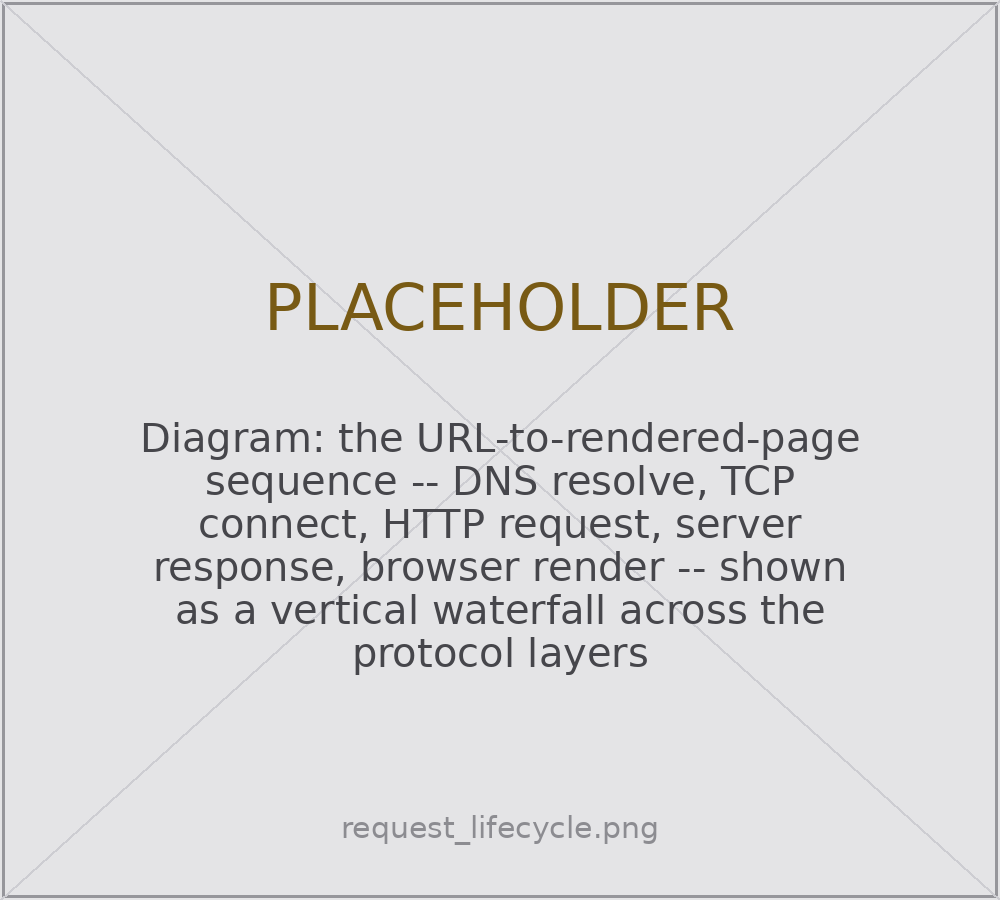
\includegraphics[width=\textwidth]{img/request_lifecycle.png}\\
            {\scriptsize URL to rendered page, one layer at a time.}
        \end{column}
    \end{columns}
\end{frame}

\begin{frame}{The lower stack: client--server, TCP/IP \& DNS}
    \begin{columns}[T]
        \begin{column}{0.6\textwidth}
            Every scrape and API call is one \textbf{request--response} cycle: a \textbf{client} (your browser, your Python script) asks a \textbf{server} for a resource.

            \bigskip

            \textbf{TCP/IP --- the transport.} Every machine on a public network has an IP address. Data is broken into packets, which hop across different router to router paths, and are re-assembled on arrival.
            \bigskip

            \textbf{DNS --- the address book.} It maps a name like \texttt{en.wikipedia.org} to an IP. Names are hierarchical --- \texttt{subdomain.domain.TLD} --- and services follow conventions: \texttt{api.agency.gov}, \texttt{data.agency.gov}.
        \end{column}
        \begin{column}{0.35\textwidth}
            \centering
            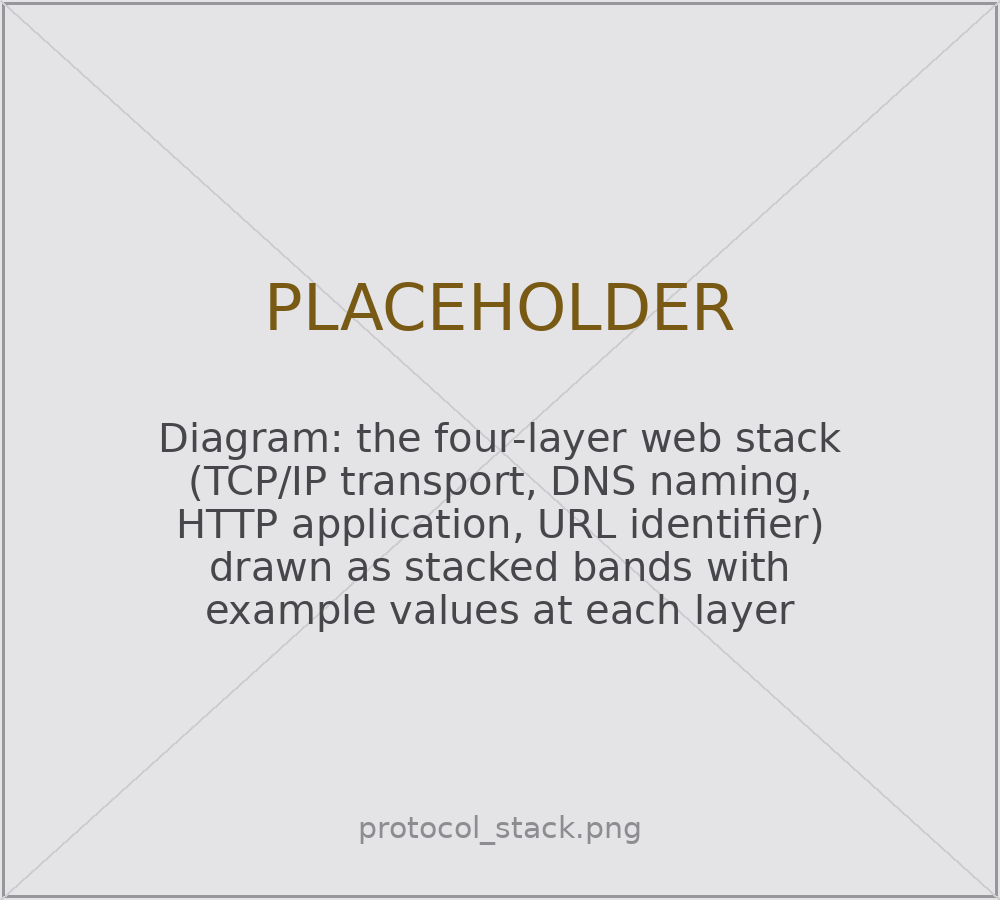
\includegraphics[width=\textwidth]{img/protocol_stack.png}
        \end{column}
    \end{columns}
\end{frame}

\begin{frame}{Inspecting a page: the Inspector tab}
    Before writing a line of code, inspect the page by hand. Open dev tools with \texttt{Ctrl+Shift+I} or \texttt{F12} (\texttt{Cmd+Opt+I} on a Mac) --- or faster: \textbf{right-click the exact thing you care about} and choose \textbf{Inspect} (Chrome, Firefox) or \textbf{Inspect Element} (Safari). This jumps straight to that element instead of the top of a page that might be thousands of lines long.

    \medskip

    \begin{itemize}\small 
        \item What you see is the ``document object model'' --- the page \emph{after} JavaScript finished making it look nicer.
        \item ``View Source'' shows the original bytes --- if an element is in the Inspector but missing from \texttt{requests.get(url).text}, JavaScript put it there.
        \item \textbf{Hover} a node to highlight it on the page
        \item Right-click a node for \textbf{Copy selector} / \textbf{Copy XPath} --- a working starting point for \texttt{soup.select()}, though often longer than it needs to be.
        \item Edits here are local and temporary --- safe to delete a cookie banner and see the structure beneath.
    \end{itemize}

    \medskip
    Start on a plain Wikipedia article --- commercial sites bury structure under tracking scripts.
\end{frame}

\begin{frame}{Inspecting a page: what the Inspector shows}
    \centering
    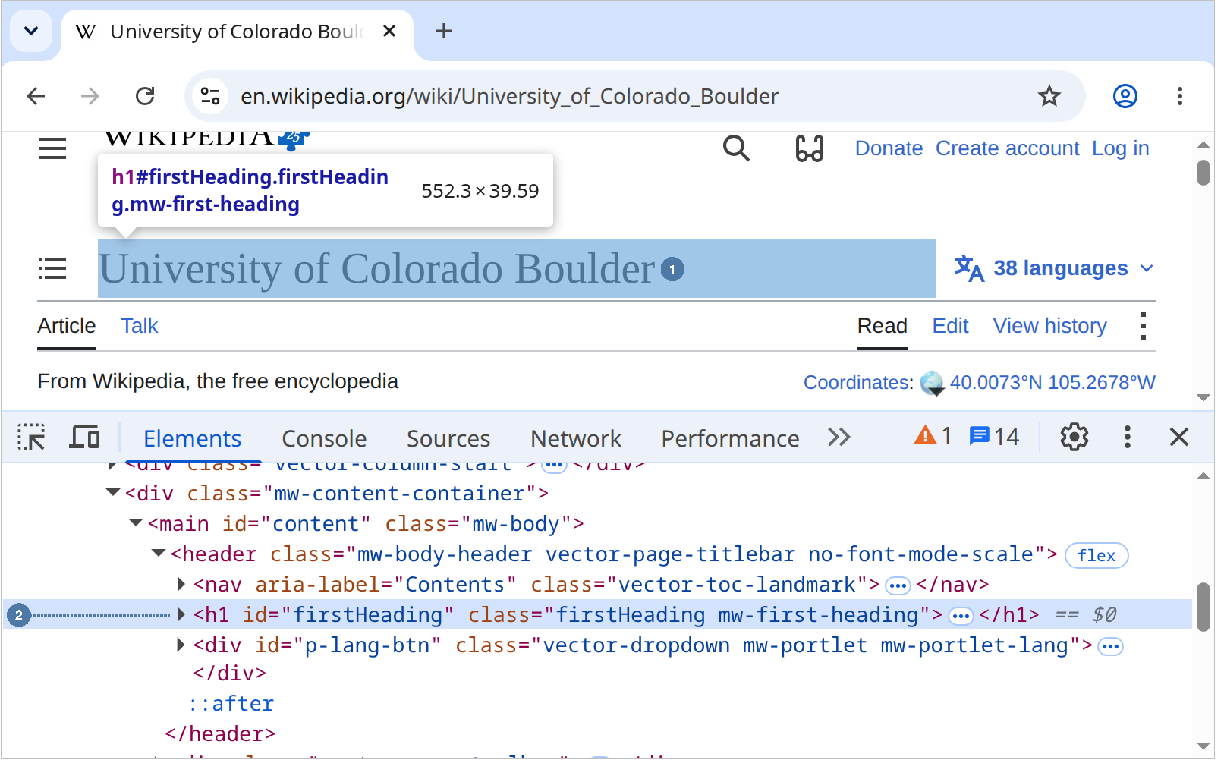
\includegraphics[width=0.75\textwidth]{img/inspector-heading_annotated.pdf}\\
    {\scriptsize Hover a node (2) and the browser shades its element on the page (1), labeled with its tag, \texttt{id}, classes, and size. Wikipedia, September 2026.}
\end{frame}

\begin{frame}{Inspecting requests: the Network tab}
    \begin{columns}[T]
        \begin{column}{0.6\textwidth}
            Click the \textbf{Network} tab. Reload \emph{after} opening it.

            \bigskip
            A page load is dozens or hundreds of requests: HTML, CSS, JS, images, trackers. 
            
            \bigskip
            Each row shows Name, Status, Type, Size, etc.

            \bigskip

            Click a request for \textbf{Headers} (incl.\ \texttt{User-Agent}, \texttt{Cookie}), \textbf{Response} (the raw JSON), and \textbf{Timing}. 

            \bigskip
            Right-click \textbf{Copy} $\to$ \textbf{Copy as cURL} reproduces the exact request --- headers, cookies, body.
        \end{column}
        \begin{column}{0.35\textwidth}
            \centering
            
\includegraphics[width=\textwidth]{slides/week-05/img/network-requests-inspector.png}\\
            {\scriptsize One page load, dozens of requests.}
        \end{column}
    \end{columns}
\end{frame}

\begin{frame}{Domain names aren't all \texttt{.com}}
    \begin{columns}[T]
        \begin{column}{0.55\textwidth}
            Most of this chapter's examples end in \texttt{.org}, \texttt{.gov}, or \texttt{.edu} --- a U.S.-centered artifact of who built the early internet.

            \bigskip

            The U.S.\ has its own country-code TLD, \texttt{.us} that no one uses: \texttt{www.sos.state.co.us/}

            \bigskip
            
            \bigskip
            Most other countries went the opposite way: \texttt{bbc.co.uk}, \texttt{spiegel.de}, \texttt{rakuten.co.jp}
        \end{column}
        \begin{column}{0.4\textwidth}
            \begin{block}{Two wrinkles to recognize}
                \footnotesize
                \textbf{Repurposed TLDs.} \texttt{.io} (British Indian Ocean Territory $\to$ ``input/output''), \texttt{.ai} (Anguilla $\to$ AI startups), \texttt{.tv} (Tuvalu $\to$ streaming)

                \medskip

                \textbf{Non-Latin domains.} DNS is ASCII-only but a common attack vector
            \end{block}
        \end{column}
    \end{columns}
\end{frame}

\begin{frame}{The upper stack: HTTP status codes \& URLs}
    \begin{center}
        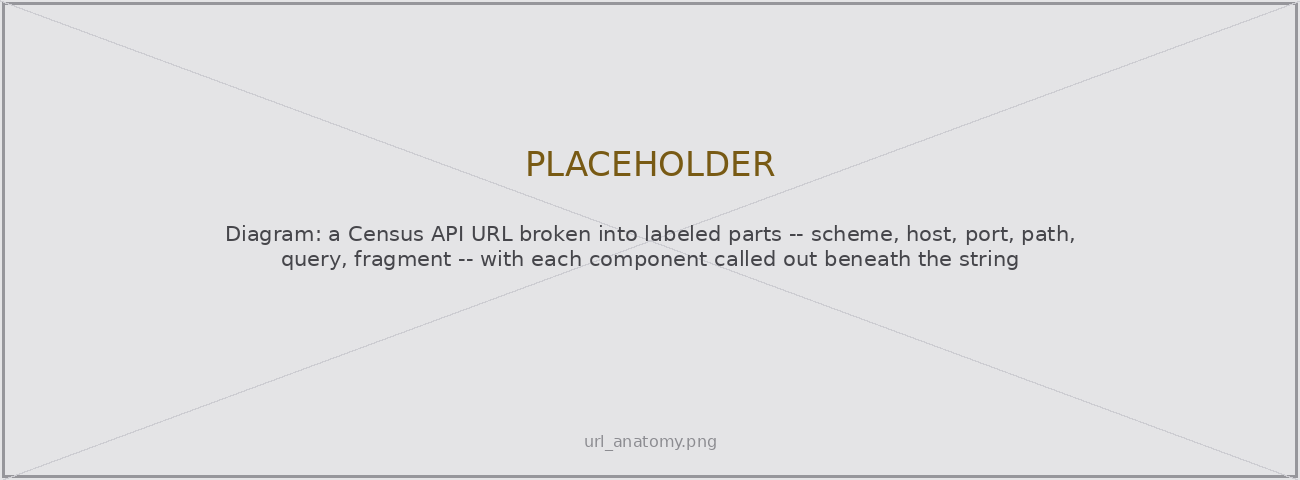
\includegraphics[width=.75\textwidth]{img/url_anatomy.png}
    \end{center}
    
    \textbf{HTTP} structures the conversation: a request carries a method (GET, POST, \dots) and headers; a response carries a \textbf{status code}:
    \begin{itemize}\small
        \item \textbf{200} OK --- the body has your data
        \item \textbf{301/302} redirect --- follow \texttt{Location}
        \item \textbf{403} forbidden --- often a missing \texttt{User-Agent}
        \item \textbf{404} not found \quad \textbf{429} slow down
        \item \textbf{500} the server's problem, not yours
    \end{itemize}
    
    The Network tab's \textbf{Status} column already shows you these, before you open a notebook.
\end{frame}

\begin{frame}{User-Agent spoofing}
    \begin{columns}[T]
        \begin{column}{0.6\textwidth}
            Every request so far has identified \emph{honestly} --- \texttt{WebDataScience/1.0 (you@colorado.edu)}. 
            
            \bigskip
            \textbf{Spoofing} means sending a \texttt{User-Agent} that claims to be a browser or device you are not.

            \bigskip
            {\footnotesize \texttt{Mozilla/5.0 (Macintosh; Intel Mac OS X 10.15; rv:155.0) Gecko/20100101 Firefox/155.0}}
            
            \bigskip
            Defeating a site's stated block with a spoofed user-agent has CFAA/ToS liability from Ch.~2.

            \bigskip
            A changed \texttt{User-Agent} string alone is weak and easily noticed

            \bigskip
            Identify yourself honestly; treat a block as a signal to stop
        \end{column}
        \begin{column}{0.35\textwidth}
            \centering\footnotesize
            
\includegraphics[width=\textwidth]{slides/week-05/img/how-do-you-do.jpeg}
            How do you do fellow browsers?
        \end{column}
    \end{columns}
\end{frame}

\begin{frame}{Closing activity: inspection patterns across real sites}
    \begin{columns}[T]
        \begin{column}{0.6\textwidth}\small
            \begin{enumerate}
                \item Pick one plain site (a Wikipedia article, a blog) and one busy site (news, ecommerce, social feed)
                \item Explore each with the Inspector: \texttt{data-*} attributes, how deep the nesting gets before you get to text, class names that look hand-written vs.\ auto-generated
                \item Explore each with Network: how many requests are needed to load a page, what kinds of files and errors, are some requests going to other domains?
                \item Find one value or attribute and edit it inside the Inspector to see it render on the page
                \item Find one annoying thing --- a cookie banner, a paywall overlay --- and delete it live. Note what it looked like before and after
            \end{enumerate}

            \bigskip
            Report back with some gnarly examples
        \end{column}
        \begin{column}{0.35\textwidth}
            
\includegraphics[width=\textwidth]{slides/week-05/img/ptsd.jpg}
        \end{column}
    \end{columns}
\end{frame}

% =========================================================================
\section{Wednesday · Notebook Lab}
% =========================================================================

\begin{frame}[fragile]{Locating yourself and the server}
    Your public IP is how the internet sees you; DNS is how a name becomes a routable address:
\begin{lstlisting}[basicstyle=\normalsize\ttfamily]
import requests
import dns.resolver

# Your public IP, as servers on the internet see it
print(requests.get("https://api.ipify.org?format=json").json())
# {'ip': '128.138.xxx.xxx'}

# Resolve a domain name to its IP address(es)
for rec in dns.resolver.resolve("en.wikipedia.org", "A"):
    print("IP address:", rec)
\end{lstlisting}
    Before reaching for Python, \texttt{ping en.wikipedia.org} from any terminal is the fastest reachability check --- no install required, works on every platform.
\end{frame}

\begin{frame}[fragile]{Getting \texttt{scapy} running: the sudo dance}
    \texttt{scapy} sends and receives raw packets --- a privileged OS operation everywhere, unrelated to \texttt{scapy} itself. Skipping these steps is the \#1 way to get stuck:
\begin{lstlisting}[language=]
1. pip install scapy          # or: conda install -c conda-forge scapy
2. Windows only: install Npcap (a driver, not a pip package)
3. Launch Jupyter WITH ELEVATED PRIVILEGES:
     macOS/Linux:  sudo jupyter notebook
     Windows:      Anaconda Prompt -> right-click -> Run as administrator
\end{lstlisting}
    \begin{alertblock}{Two gotchas}
        \footnotesize \texttt{sudo} resets your shell's \texttt{PATH} --- a bare \texttt{sudo jupyter notebook} can launch the \emph{wrong} Jupyter and fail with \texttt{ModuleNotFoundError}. Fix: \texttt{sudo \$(which jupyter) notebook}. And: an elevated notebook gives \emph{every} cell full system access, not just the one that needs it --- close it when you're done. Machine won't cooperate? The terminal backup on the next frame needs no privileges at all.
    \end{alertblock}
\end{frame}

\begin{frame}[fragile]{Traceroute: reading the hops}
\begin{lstlisting}
from scapy.all import traceroute

result, unans = traceroute("en.wikipedia.org", maxttl=20)
\end{lstlisting}
    Each line is one hop --- an IP (or hostname) and a round-trip time. Patterns worth recognizing:
    \begin{itemize}\small
        \item \texttt{* * *} --- an unanswered hop, not a broken path; many routers rate-limit or drop probes on purpose
        \item Private IPs (\texttt{10.}, \texttt{192.168.}, \texttt{172.16--31.}) in the first hop or two --- your own network, normal
        \item A sudden RTT jump --- often a long-haul or undersea link, not a problem
        \item Hostnames often encode geography (\texttt{iad}, \texttt{ord}) --- a fast, informal location guess
    \end{itemize}
    \footnotesize No privileges needed: \texttt{traceroute en.wikipedia.org} (macOS/Linux) or \texttt{tracert en.wikipedia.org} (Windows) from any terminal.
\end{frame}

\begin{frame}[fragile]{Packet sniffing: watching your own traffic}
    Every message in this chapter travels as \textbf{packets}. \textbf{Sniffing} captures them off an interface --- meaningfully more invasive than anything else here, so this book sniffs only \textbf{loopback traffic you generate yourself}, to a server on your own machine:
\begin{lstlisting}
from scapy.all import AsyncSniffer
import requests, threading
from http.server import HTTPServer, SimpleHTTPRequestHandler

httpd = HTTPServer(("127.0.0.1", 8899), SimpleHTTPRequestHandler)
threading.Thread(target=httpd.serve_forever, daemon=True).start()

sniffer = AsyncSniffer(filter="tcp port 8899", iface="lo0")  # "lo" on Linux
sniffer.start()
requests.get("http://127.0.0.1:8899/")
packets = sniffer.stop()

for pkt in packets:
    print(pkt.summary())
\end{lstlisting}
    \footnotesize The first packets are TCP's \textbf{handshake} --- \texttt{SYN}, \texttt{SYN-ACK}, \texttt{ACK} --- before a byte of your actual request goes out. Prefer clicking to scripting? \textbf{Wireshark} is the standard GUI packet analyzer, same idea, no code.
\end{frame}

\begin{frame}[fragile]{Diagnosing HTTP errors, not guessing}
    The status code says \emph{what} failed; the full response says \emph{why}. Read both:
\begin{lstlisting}
def diagnose_request(url, headers=None):
    try:
        r = requests.get(url, headers=headers, timeout=10)
    except requests.exceptions.ConnectionError:
        return print("Connection failed:", url)
    print("Status:", r.status_code)
    print("Content-Type:", r.headers.get("Content-Type", "n/a"))
    print("Bytes:", len(r.content))
    if r.history:                       # a redirect chain
        print("Redirected from:", r.history[0].url)
    return r
\end{lstlisting}
    A \textbf{403} from an API usually means a missing \texttt{User-Agent} (a one-line fix); a \textbf{403} from a news site may block scraping outright. A \textbf{429} means slow down; a \textbf{500} is the server's problem --- retry later.
\end{frame}

\begin{frame}[fragile]{Make an API call, get a time series}
    \begin{columns}[T]
        \begin{column}{0.6\textwidth}
        The Wikimedia pageviews API rejects the default client with \textbf{403} --- add a meaningful \texttt{User-Agent} and it returns \textbf{200}:
\begin{lstlisting}
url = ("https://wikimedia.org/api/rest_v1/"
       "metrics/pageviews/per-article/en.wikipedia/"
       "all-access/all-agents/"
       "University_of_Colorado_Boulder/daily/"
       "20260101/20260131")
ua = {"User-Agent": "WebDataScience/1.0 (you@colorado.edu)"}
data = requests.get(url, headers=ua).json()
\end{lstlisting}
        Reshape the nested JSON, then plot it:
\begin{lstlisting}
df = pd.DataFrame(data["items"])
df["timestamp"] = pd.to_datetime(df["timestamp"],
                                 format="%Y%m%d00")
df.plot(x="timestamp", y="views")
\end{lstlisting}
        \end{column}
        \begin{column}{0.35\textwidth}
            \centering
            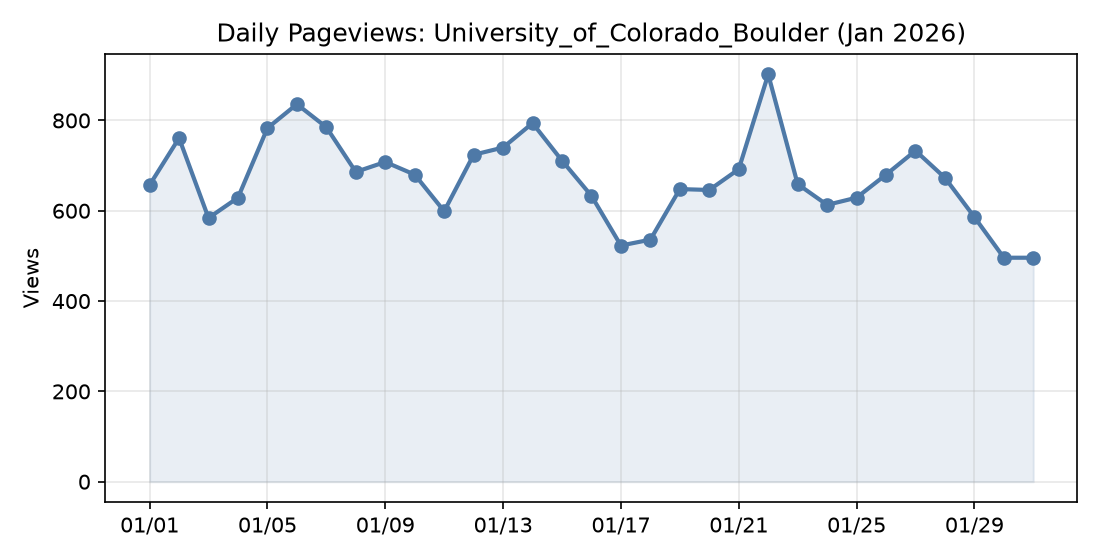
\includegraphics[width=\textwidth]{img/pageviews_timeseries.png}\\
            {\scriptsize Daily pageviews --- spikes line up with real-world events.}
        \end{column}
    \end{columns}
\end{frame}

\begin{frame}[fragile]{User-Agent spoofing, mechanically}
    Spoofing is just the \texttt{headers} dict you already know --- with a value describing a browser you are not:
\begin{lstlisting}
honest = {"User-Agent": "WebDataScience/1.0 (you@colorado.edu)"}
spoofed = {"User-Agent": (
    "Mozilla/5.0 (Windows NT 10.0; Win64; x64) AppleWebKit/537.36 "
    "(KHTML, like Gecko) Chrome/128.0.0.0 Safari/537.36"
)}

# httpbin.org just echoes back whatever header you sent --
# a safe way to see exactly what a server receives
print(requests.get("https://httpbin.org/user-agent", headers=honest).json())
print(requests.get("https://httpbin.org/user-agent", headers=spoofed).json())
\end{lstlisting}
    You already saw this header change real behavior earlier today: the pageviews API's default client got \textbf{403}; a named one got \textbf{200}. Same mechanism, different intent.
\end{frame}

\begin{frame}[fragile]{A loop over one host is your cue for a Session}
    A bare \texttt{requests.get()} opens a fresh connection every time. Looping over many URLs at one host? Create a \texttt{Session} --- it reuses the connection, remembers headers, and retries automatically:
\begin{lstlisting}
from requests.adapters import HTTPAdapter
from urllib3.util.retry import Retry

session = requests.Session()
session.headers.update({"User-Agent": "WebDataScience/1.0 (you@colorado.edu)"})

# Retry 429/5xx with backoff of 1s, 2s, 4s; honors Retry-After
retries = Retry(total=3, backoff_factor=1,
                status_forcelist=[429, 500, 502, 503, 504])
session.mount("https://", HTTPAdapter(max_retries=retries))

for article in ["Web_scraping", "Data_science"]:
    r = session.get(f"https://en.wikipedia.org/wiki/{article}")
\end{lstlisting}
    Six lines of setup replace the hand-rolled backoff loop --- and carry over unchanged into the scraping, Wikipedia, and government-data chapters.
\end{frame}

\begin{frame}[fragile]{The same requests, from the terminal}
    Every Python lookup so far has a direct terminal equivalent --- no install beyond what your OS already ships:
\begin{lstlisting}[language=]
dig en.wikipedia.org              # or: nslookup en.wikipedia.org (any OS)
  -> same A record as dns.resolver, plus which server answered and its TTL

whois wikipedia.org
  -> a different question than DNS: who registered this, and when

curl -I https://en.wikipedia.org  # headers only -- fast status check
curl -v https://en.wikipedia.org  # full request/response, like the Network tab
\end{lstlisting}
    All four take a User-Agent flag (\texttt{curl -A "..."}) the same way the \texttt{headers} dict does in Python.
\end{frame}

\begin{frame}[fragile]{\texttt{curl} and \texttt{wget}: alternatives to \texttt{requests}}
    Every tool in this section fetches; \textbf{neither parses}. The moment you need JSON, HTML, or a DataFrame, you are back to \texttt{requests}. They earn their place for a one-off check, a shell script, a server with no Python, or saving straight to disk.

    \medskip

    \texttt{curl} is built for control (headers, methods, auth); \texttt{wget} is built for downloading (saves to disk automatically, resumes, rate-limits). Setting a User-Agent, either way:
\begin{lstlisting}[language=]
curl -A "WebDataScience/1.0 (you@colorado.edu)" https://en.wikipedia.org/wiki/Web_scraping
wget --user-agent="WebDataScience/1.0 (you@colorado.edu)" https://en.wikipedia.org/wiki/Web_scraping
\end{lstlisting}
    \footnotesize \texttt{curl} prints to your terminal by default (\texttt{-O} saves to a file); \texttt{wget} always saves to disk.
\end{frame}

\begin{frame}[fragile]{Replicating \texttt{sleep()}, and fetching many files}
    \texttt{wget} has rate-limiting \textbf{built in}; \texttt{curl} does not:
\begin{lstlisting}[language=]
wget --wait=2 --random-wait URL1 URL2
  -> jitters 0.5x-1.5x of --wait automatically

for url in URL1 URL2; do curl -O "$url"; sleep 2; done
  -> curl needs a shell loop -- the terminal version of time.sleep()
\end{lstlisting}
    A known list of files, one call, rate-limited for free:
\begin{lstlisting}[language=]
wget -i articles.txt --wait=2 --random-wait \
     --user-agent="WebDataScience/1.0 (you@colorado.edu)"
\end{lstlisting}
    \footnotesize Same task as this morning's \texttt{Session} loop over three articles --- a text file of URLs instead of a Python list.
\end{frame}

\begin{frame}[fragile]{Parse --- and build --- URLs with the right tool}
    Never parse a URL with a regular expression. \texttt{urllib.parse} follows the spec:
\begin{lstlisting}
from urllib.parse import urlparse, parse_qs, quote

u = urlparse("https://api.census.gov/data/2022/acs/acs5?get=NAME&for=place:07850")
u.scheme, u.netloc, u.path   # 'https', 'api.census.gov', '/data/2022/acs/acs5'
parse_qs(u.query)            # {'get': ['NAME'], 'for': ['place:07850']}
\end{lstlisting}
    Two API styles need two builders. \textbf{Path-segment} APIs need \texttt{quote()} on each component; \textbf{query-parameter} APIs take a \texttt{params=} dict and let \texttt{requests} do the escaping:
\begin{lstlisting}
quote("AC/DC", safe="")   # 'AC%2FDC' -- the slash MUST be encoded
requests.get(base, params={"titles": "University of Colorado Boulder"})
\end{lstlisting}
    Mixing them up --- query-encoding a value the API expects in its path --- is a classic source of confusing 404s.
\end{frame}

\begin{frame}{Lab: work these, then show-and-tell}
    \begin{columns}[T]
        \begin{column}{0.6\textwidth}
            Work in pairs. Do these exercises from the chapter:
            \begin{enumerate}\small
                \item Open the Network tab on a Wikipedia article and on a news site. Count the requests. Give the fraction that is content and the fraction that is tracking.
                \item Resolve five related domains with \texttt{dns.resolver}. Report the domains that share an IP address.
                \item Plot the pageviews of three related articles. Give a possible cause for each spike.
                \item Write \texttt{diagnose\_url()}. Test it on a 200 response, a 404 response, a redirect, an API, and a blocked site.
                \item Run the packet-sniffer cell against your own loopback request. Identify the \texttt{SYN}, \texttt{SYN-ACK}, and \texttt{ACK} packets in the output.
                \item \textbf{5617:} examine the delivery infrastructure of one site. Record the redirect chain, the CDN headers, and the traceroute hops. Write a 500-word memo
            \end{enumerate}
        \end{column}
        \begin{column}{0.35\textwidth}
            \begin{block}{Show-and-Tell}
                \footnotesize Bring one of these to class:
                \begin{itemize}\footnotesize
                    \item a bug that you could not solve
                    \item data that you collected and find interesting
                    \item a question for a research design
                \end{itemize}
            \end{block}
        \end{column}
    \end{columns}
\end{frame}

\begin{frame}[standout]
    When a request fails, don't guess.\\
    Ask the stack, in order:\\[0.8em]
    {\large Can I reach the server?\\
    Am I resolving the right address?\\
    What status code came back?\\
    Are my headers correct?\\
    Is my URL well-formed?}
\end{frame}

% =========================================================================
\section{Friday · Textbook Revisions}
% =========================================================================

\begin{frame}{Improving Chapter 5 together}
    \begin{columns}[T]
        \begin{column}{0.48\textwidth}
            Today we make the book better. Each of you opens a \textbf{pull request} against \texttt{ch-05-protocols.qmd} and reviews a classmate's.

            \medskip

            \textbf{The workflow} (from Week 1):
            \begin{enumerate}\footnotesize
                \item Branch / fork the book repo
                \item Edit the chapter; commit with a clear message
                \item Open a PR describing \textit{what} and \textit{why}
                \item Review two peers' PRs: kind, specific, actionable
            \end{enumerate}
        \end{column}
        \begin{column}{0.5\textwidth}
            \begin{block}{A strong PR}
                \footnotesize
                \begin{itemize}\footnotesize
                    \item One focused change, clearly titled; explains the problem it fixes
                    \item Builds (\texttt{quarto render}) without errors; matches the book's voice
                    \item Discloses any AI assistance
                \end{itemize}
            \end{block}
            \begin{block}{A strong review}
                \footnotesize
                \begin{itemize}\footnotesize
                    \item Runs / reads the change, not just skims; names specifics (line, claim, code)
                    \item Separates ``must fix'' from ``nice to have''; generous, ends with a clear verdict
                \end{itemize}
            \end{block}
        \end{column}
    \end{columns}
\end{frame}

\begin{frame}{A revision menu for Chapter 5}
    \begin{columns}[T]
        \begin{column}{0.6\textwidth}
            High-value targets --- pick one and scope it to a single PR:
            \begin{itemize}\footnotesize
                \item \textbf{Test the code against live services.} \texttt{ipify}, \texttt{ip-api.com} (45 req/min), the Wikimedia pageviews API, and DNS results all drift. Run the notebook, report what broke, and fix it.
                \item \textbf{Add a figure.} The chapter still has zero diagrams --- a layered-stack or annotated Network-tab figure would anchor the concepts.
                \item \textbf{Deepen ``Common Issues to Debug.''} An IPv6 \texttt{AAAA} lookup, and a \texttt{curl}/\texttt{wget}-specific gotcha, are still missing.
                \item \textbf{Strengthen an exercise.} Give \texttt{diagnose\_url()} expected output, a rubric, or a starter cell so it is self-checking.
                \item \textbf{Add a missing citation.} ICANN, Verisign, and \texttt{ip-api.com} are all named in the chapter without a link.
            \end{itemize}
        \end{column}
        \begin{column}{0.35\textwidth}
            \centering
            
\includegraphics[width=\textwidth]{img/pr_review.png}\\
            {\scriptsize A real review comment on a real PR.}
        \end{column}
    \end{columns}
    \medskip
    \centering\small Next week: \textbf{Parsing static web pages} --- turning messy HTML into a clean DataFrame.
\end{frame}

% =========================================================================
\begin{frame}{Key takeaways}
    \begin{enumerate}\small
        \item The web is a \textbf{layered stack}: TCP/IP transports, DNS resolves names, HTTP structures the conversation, URLs identify the target.
        \item \textbf{Traceroute and packet sniffing} make that transport layer directly observable; the \texttt{User-Agent} header --- honest or spoofed --- is how a server decides who, or what, is asking.
        \item Debugging is \textbf{systematic diagnosis}, not guesswork: reach the server? right address? which status code? headers correct? URL well-formed?
        \item A meaningful \texttt{User-Agent} fixes most \textbf{403}s; backoff or a \texttt{Retry} policy handles \textbf{429}s. A \texttt{for} loop over one host is your cue for a \texttt{Session}.
        \item \textbf{Never regex a URL.} \texttt{urllib.parse} both parses and builds; know path-segment (\texttt{quote}) from query-parameter (\texttt{params=}) APIs.
        \item \texttt{requests} has a terminal equivalent in \texttt{curl} and \texttt{wget} --- know when opening a notebook is more overhead than the task deserves.
    \end{enumerate}
    \bigskip
\end{frame}

\end{document}
